\documentclass{astroedu-lab}

\begin{document}

\pagestyle{plain}

\begin{problem}{\huge Лабораторная работа 5.1.1\\\\Экспериментальная проверка\\\\ уравнения Эйнштейна\\\\
для фотоэффекта\\\\Выполнил Жданов Елисей Б01-205}

\section{Цель работы:}

Исследовать зависимость фототока от величины задерживающего потенциала и частоты падающего излучения, что позволяет вычислить величину постоянной Планка.
	

\section{Теоретическая справка}

Фотоэффект --- явление испускания электронов фотокатодом, облучаемым светом. Энергетический баланс этого взаимодействия для вылетающих электронов описывается уравнением
	
	\begin{equation}\label{energy balance}
	\hbar \omega = E_{max} + W
	\end{equation}
	

	
	Здесь $ E_{max} $ ---  максимальная кинетическая энергия электрона после выхода из фотокатода, $ W $ --- работа выхода электрона из катода. Энергетический спектр вылетевших из фотокатода электронов непрерывен --- он простирается от нуля до $ E_{max} $. 
	
	\begin{figure}[!h]
	\centering
	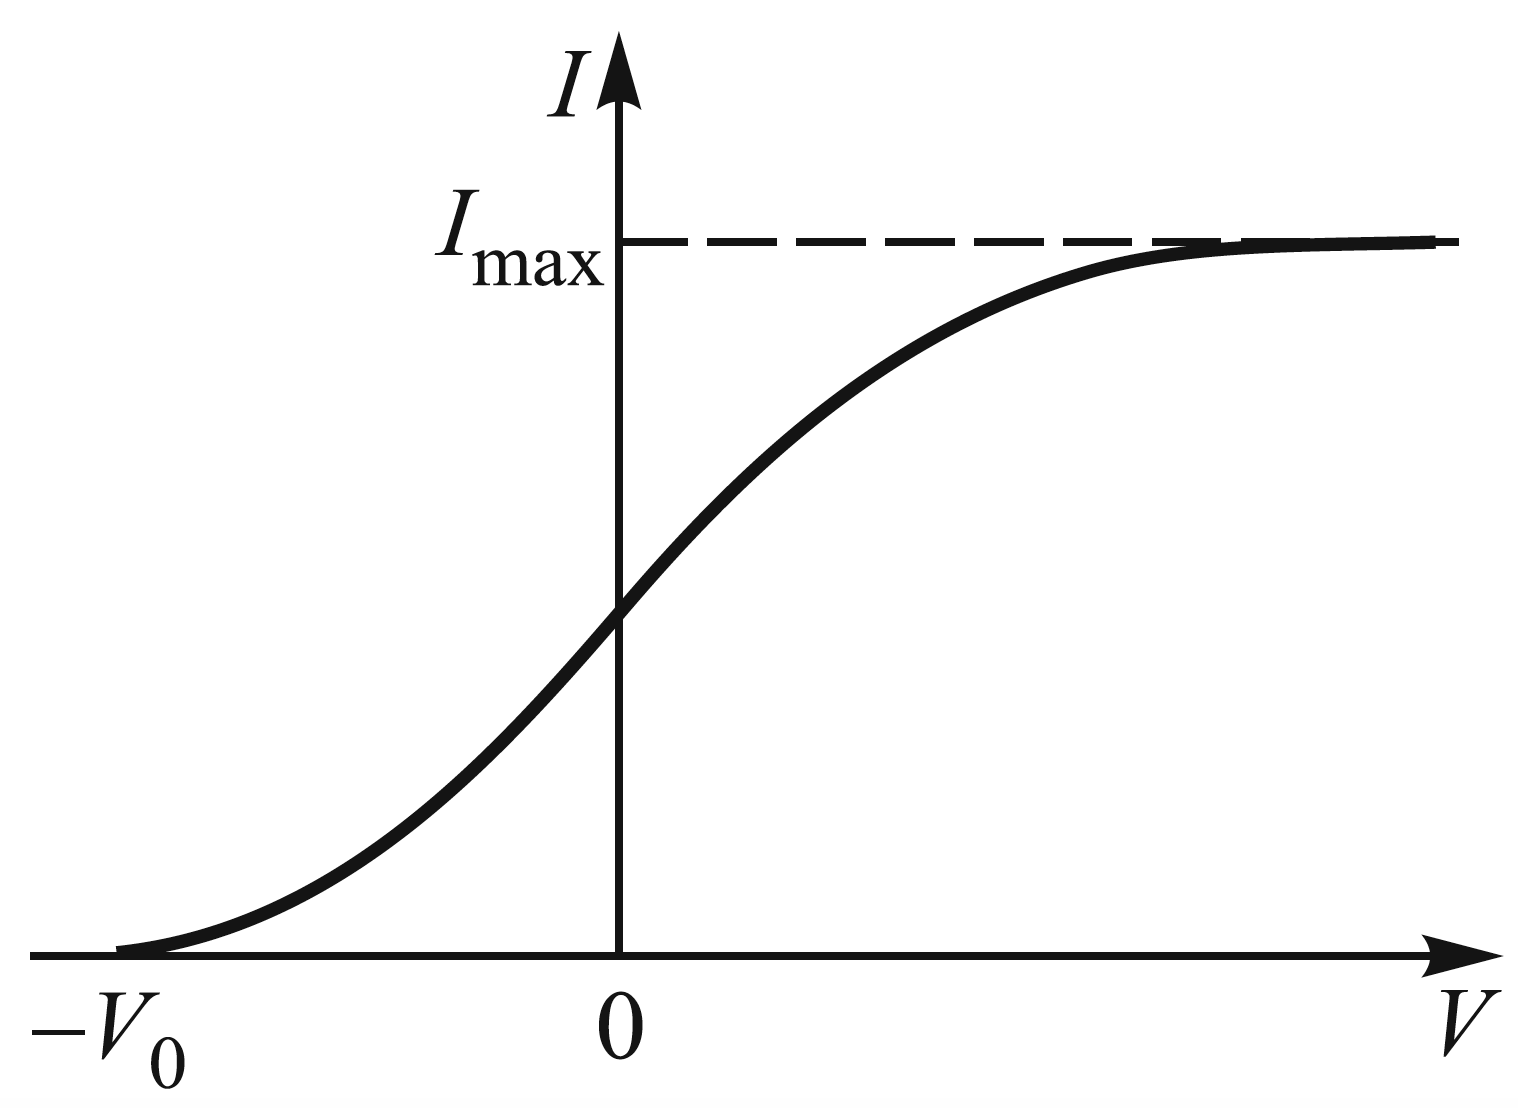
\includegraphics[width=0.3\linewidth]{I(V)}
	\caption{Зависимость фототока от напряжения на аноде фотоэлемента}
	\label{ris I(V)}
\end{figure}
	
	Для измерения энергии вылетевших фотоэлектронов вблизи фотокатода
	обычно располагается второй электрод
	(анод), на который подается задерживающий ($ V < 0 $) или ускоряющий ($ V >
	0 $) потенциал. При достаточно больших
	ускоряющих напряжениях фототок достигает насыщения (рис. \ref{ris I(V)}): все испущенные электроны попадают на анод.
	
	При задерживающих потенциалах на анод попадают лишь электроны,
	обладающие достаточно большой кинетической энергией, в то время
	как медленно движущиеся электроны заворачиваются полем и возвращаются на катод. При некотором значении $ V = -V_0 $ (потенциал запирания) даже наиболее быстрые фотоэлектроны не могут достичь
	анода.
	Максимальная кинетическая энергия $ E_{max} $ электронов связана с
	запирающим потенциалом $ V_0 $ очевидным соотношением $ E_{max} = eV_0 $. Тогда \eqref{energy balance} примет вид, называемый уравнением Эйнштейна:
	
	\begin{equation}\label{Einsteain}
	eV_0 = \hbar\omega - W 
	\end{equation}
	
	Чтобы определить величину запирающего
	напряжения, нам надо правильно экстраполировать получаемую токовую зависимость к нулю, т. е. определить, какова функциональная
	зависимость $ I(V) $. Расчет для простейшей геометрии --- плоский катод, освещаемый светом, и параллельный ему анод --- приводит к зависимости
	
	\begin{equation}\label{sqrt I = V}
	\sqrt{I} \propto V_0 - V
	\end{equation}
	
	т. е. корень квадратный из фототока линейно
	зависит от запирающего напряжения. Эта зависимость хорошо описывает экспериментальные данные.
	
	В работе изучается зависимость фототока из фотоэлемента от величины задерживающего потенциала $ V $ для различных частот света $ \omega $, лежащих в видимой области спектра. С целью экспериментальной
	проверки уравнения Эйнштейна определяются потенциалы запирания
	$ V_0 $ при разных частотах света и строится зависимость $ V_0(\omega) $, которая, как это следует из \eqref{Einsteain}, должна иметь вид
	
	\begin{equation}\label{V(w)}
	V_0 (\omega) = \dfrac{\hbar\omega - W}{e}
	\end{equation}



	\begin{figure}[!h]
	\centering
	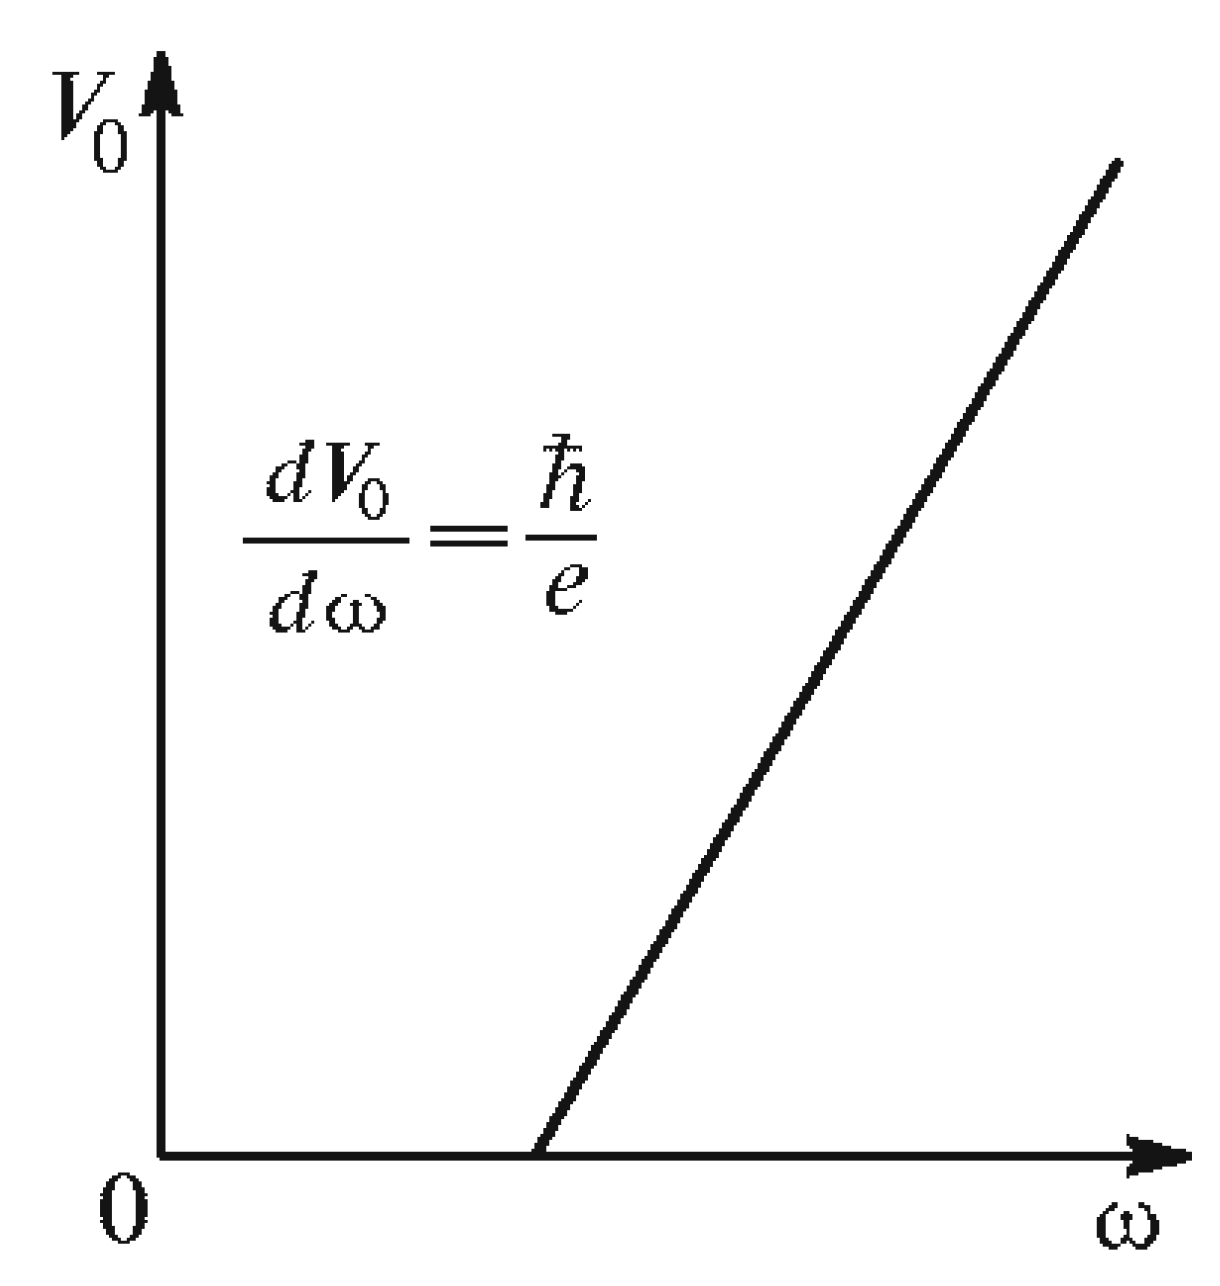
\includegraphics[width=0.3\linewidth]{V(w)}
	\caption{Зависимость запирающего потенциала
			от частоты света}
	\label{ris V(w)}
\end{figure}
	
	Потенциал запирания $ V_0 $ для любого катода линейно зависит от
	частоты света $ \omega $. По наклону прямой на графике $ V_0(\omega) $ (рис. \ref{ris V(w)}) можно определить постоянную Планка:
	
	\begin{equation}\label{dV/dw}
	\dfrac{dV_0}{d\omega} = \dfrac{\hbar}{e}
	\end{equation}
	
	Как показывает формула \eqref{dV/dw}, угол наклона прямой $ V_0(\omega) $ не зависит от рода вещества, из которого изготовлен фотокатод. От рода вещества, однако, зависит величина фототока, работа выхода $ W $ и форма кривой $ I(V) $ (рис. \ref{ris I(V)}). Все это определяет выбор пригодных для
	опыта катодов.

\section{Экспериментальная установка}

\begin{figure}[!h]
	\centering
	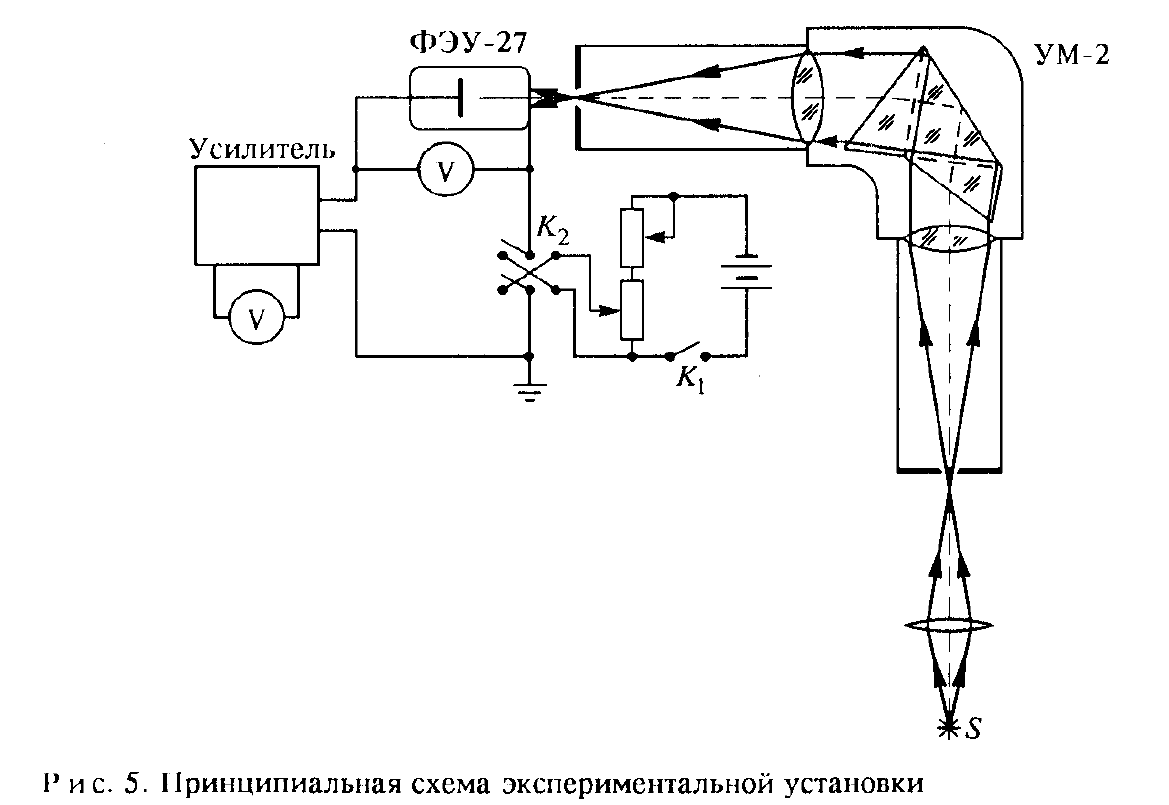
\includegraphics[width=0.9\textwidth]{2024-09-27_13-24-45.png}
	\label{fig:boiler}
\end{figure}

Схема установки приведена на рис. 5. Свет от источника $S$ (электрическая лампа накаливания) с помощью конденсора фокусируется на входную щель призменного монохроматора УМ-2, выделяющего узкий спектральный интервал, и попадает на катод фотоэлемента Ф-25.


\section{Измерения, Обработка}

1) Произведем градуировку монохроматора. Снимем зависимость длины волны света от угла $\theta$ барабана монохроматора. Построим график. Погрешность шкалы много меньше случайной погрешности выставления линии спектра неона, поэтому примем её за размер точек.

Также аппроксимируем зависимость $\lambda(\theta)$ полиномом второго порядка $(a x^2 + b x + c)$.
\\
\begin{figure}[!h]
	\centering
	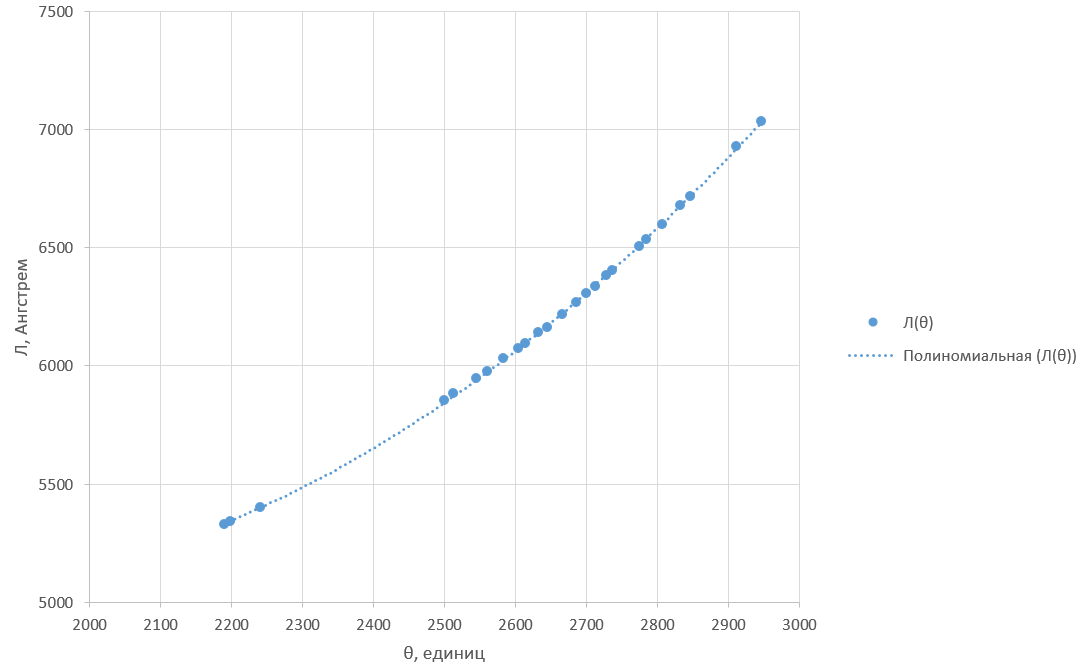
\includegraphics[width=1\textwidth]{2024-09-29_00-24-58}
	\label{fig:boiler}
\end{figure}

\begin{equation}
	y=0.0013 x^2 - 4.62 x + 9050
\end{equation}

Абсолютную погрешность по обеим осям примем равной 10 нм и единицам.

2) Опираясь на градуировку манохроматора, выполним измерения величины фототока от напряжения для разных длин волн. Значения находятся в таблице, здесь же приведем графики, линеаризованные корнем из тока по отношению к напряжению ($\sqrt{I}(U)$). 

Погрешности нанесены на график исходя из колебаний показаний фототока(порядка 10$\%$ на всем диапазоне), а также для напряжения исходя из неустойчивости работы мультиметра.


\begin{figure}[h!]
    \centering
    \begin{minipage}[b]{0.48\textwidth}
        \centering
        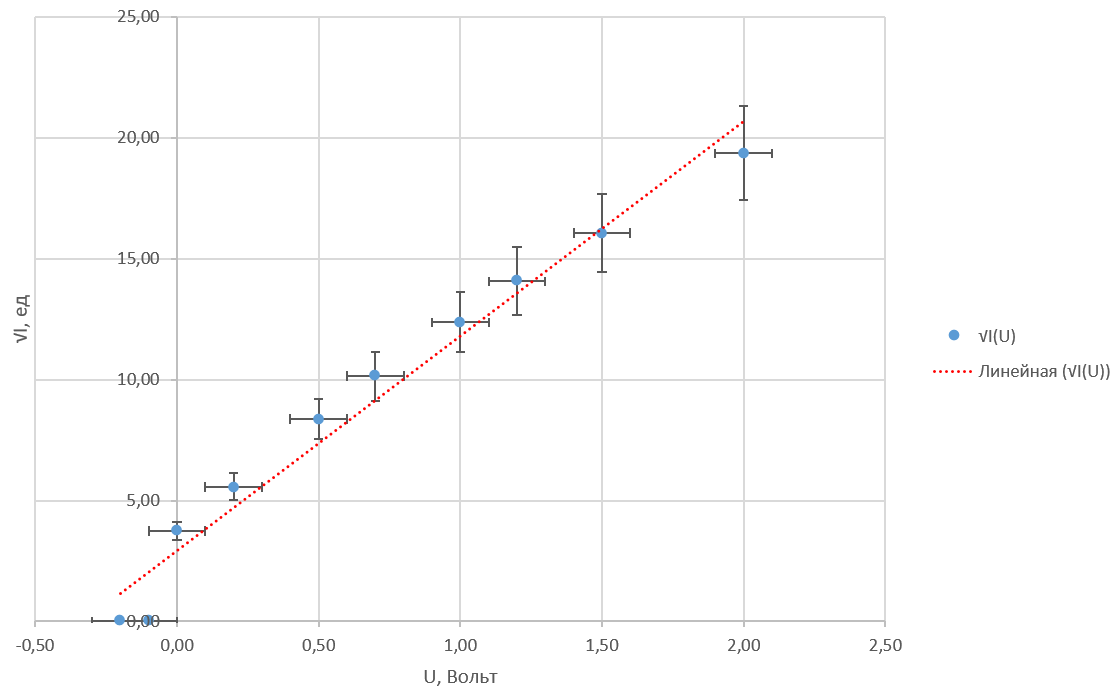
\includegraphics[width=\textwidth]{p/2024-09-29_01-12-10.png}
        \caption{$\theta = 2874^\circ$}
        \label{fig:9}
    \end{minipage}
    \hfill
    \begin{minipage}[b]{0.48\textwidth}
        \centering
        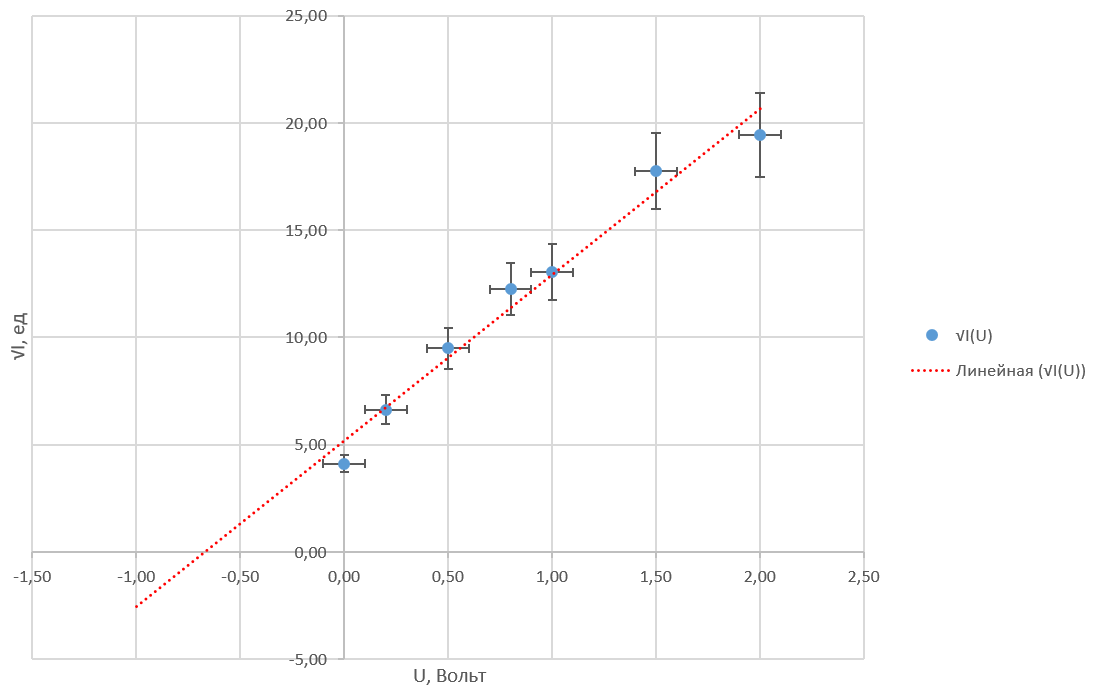
\includegraphics[width=\textwidth]{p/2024-09-29_01-15-03.png}
        \caption{$\theta = 2800^\circ$}
        \label{fig:10}
    \end{minipage}
    \hfill
    \begin{minipage}[b]{0.48\textwidth}
        \centering
        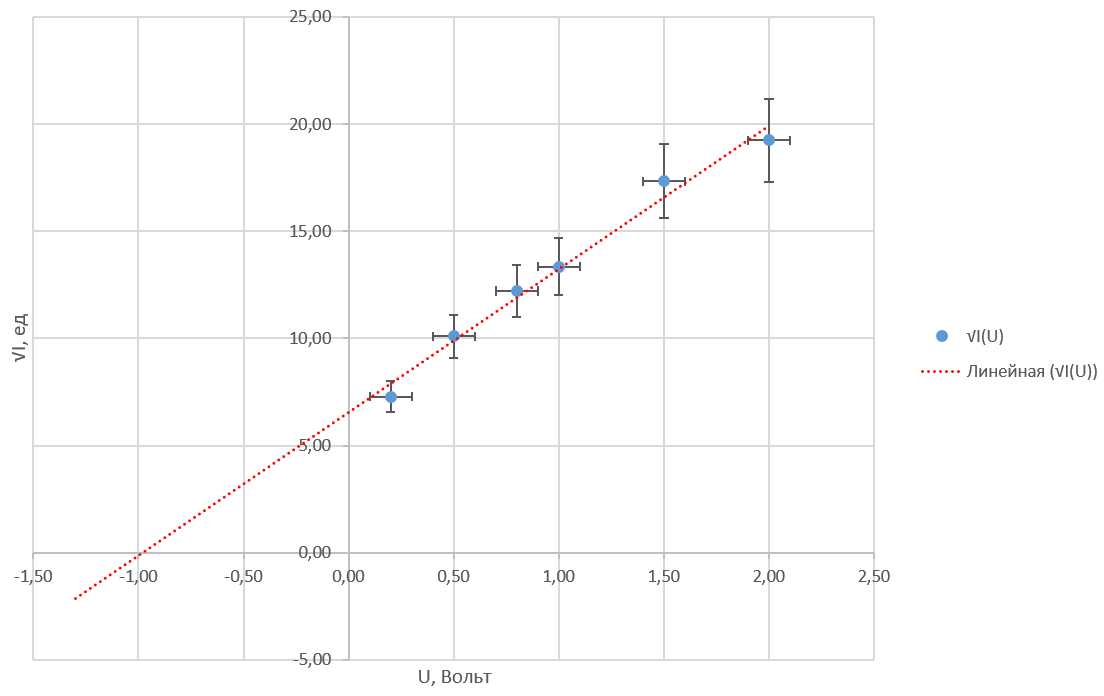
\includegraphics[width=\textwidth]{p/2024-09-29_01-18-56.png}
        \caption{$\theta = 2700^\circ$}
        \label{fig:11}
    \end{minipage}
    \hfill
    \begin{minipage}[b]{0.48\textwidth}
        \centering
        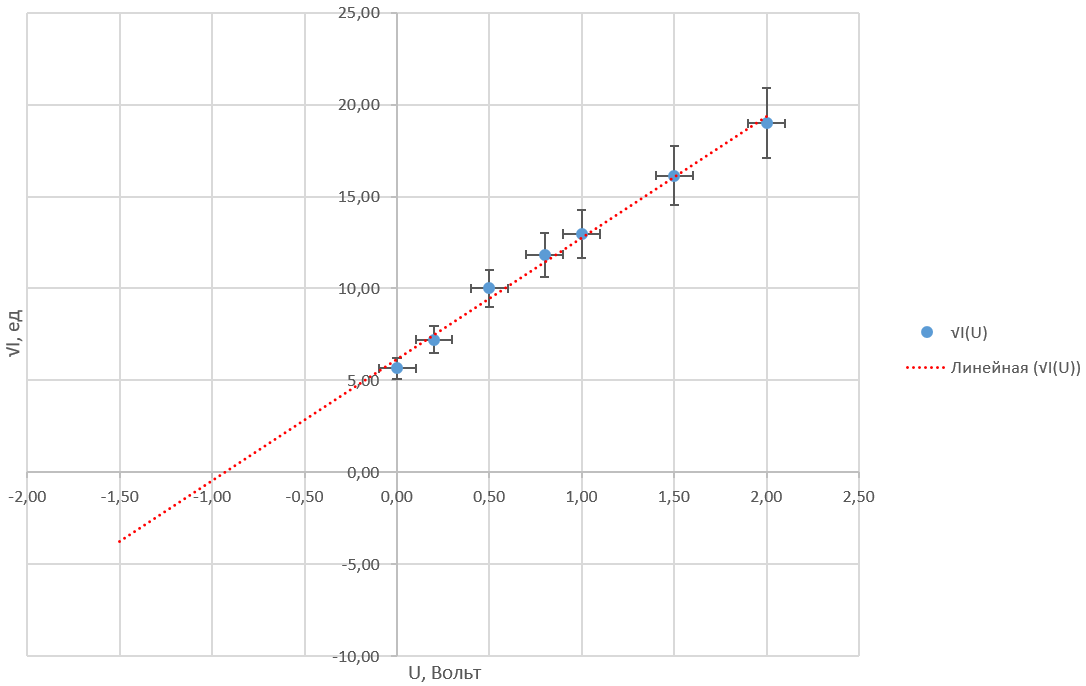
\includegraphics[width=\textwidth]{p/2024-09-29_01-21-15.png}
        \caption{$\theta = 2500^\circ$}
        \label{fig:11}
    \end{minipage}
    \hfill
    \begin{minipage}[b]{0.48\textwidth}
        \centering
        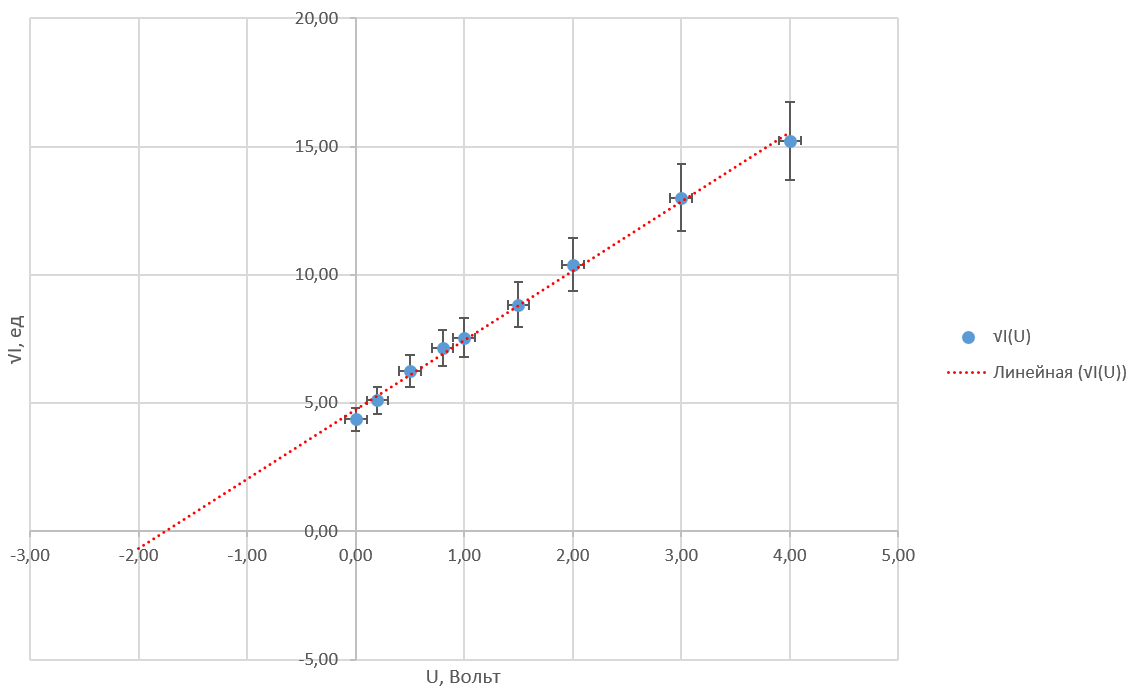
\includegraphics[width=\textwidth]{p/2024-09-29_01-24-25.png}
        \caption{$\theta = 1800^\circ$}
        \label{fig:11}
    \end{minipage}
\end{figure}


%\begin{center}
%\begin{tabular}{|c|c|c|c|}
%\hline 
%\multicolumn{2}{|c|}{$h_\text{ман}$, мм} & $\sigma, \frac{\text{мН}}{\text{К}}$ & T, $^\circ$C \\
%\hline
%\hline
%\end{tabular}
%\end{center}

%2874)y = (a ± Sa) + (b ± Sb)·x = (4.25 ± 0.26) + (7.85 ± 0.24)·x
%2800)y = (a ± Sa) + (b ± Sb)·x = (5.18 ± 0.59) + (7.74 ± 0.55)·x
%2700)y = (a ± Sa) + (b ± Sb)·x = (6.56 ± 0.49) + (6.69 ± 0.42)·x
%2500)y = (a ± Sa) + (b ± Sb)·x = (6.16 ± 0.27) + (6.6 ± 0.25)·x
%1800)y = (a ± Sa) + (b ± Sb)·x = (4.75 ± 0.13) + (2.702 ± 0.067)·x




Найдем угловые коэффициенты прямых для каждой установки по МНК.

\[
	a = \frac{<x_i y_i> - < x > < y_i >}{< x_i^2> - < x_i >^2}
\]

\[
	b = < \nu_i > - a < N_i >
\]

Также рассчитаем их погрешности

\begin{equation}
	S_a^2 = \frac{< x_i^2>}{< x_i^2 > - < x_i >^2} \cdot \frac{<  b_i - b > ^2}{n - 2}
\end{equation}

Получим следующие значения линеаризаций

\[1800) y = (4.75 \pm 0.13) + (2.70 \pm 0.07)\cdot x \]
\[2874) y = (4.3 \pm 0.3) + (7.9 \pm 0.2)\cdot x \]
\[2800) y = (5.2 \pm 0.6) + (7.7 \pm 0.6)\cdot x\] 
\[2700) y = (6.6 \pm 0.5) + (6.7 \pm 0.4)\cdot x\]
\[2500) y = (6.2 \pm 0.4) + (6.6 \pm 0.3)\cdot x \]


Из полученных аппроксимаций легко получить значение в нуле

\begin{equation}
	V_0 = -\frac{b}{a}; \varepsilon_V = \varepsilon_a \cdot \varepsilon_b
\end{equation}

Используя полученную связь угла и длины волны, подведем предварительный результат таблицей.

\begin{center}
\begin{tabular}{|c|c|c|c|}
\hline 
& $\lambda$, A & $V_0$ \\
\hline
1 & 6510 & $(-0.54 \pm 0.05)$ \\
1 & 6310 & $(-0.67 \pm 0.12)$ \\
1 & 6050 & $(-0.98 \pm 0.13)$ \\
1 & 5630 & $(-0.93 \pm 0.08)$ \\
1 & 4950 & $(-1.76 \pm 0.09)$ \\
\hline
\end{tabular}
\end{center}

Отметим также, что ток фотокатода был максимален при длине волны света 6510 нм. 

Построим график зависимости $V_0(\omega)$
	


\begin{figure}[!h]
	\centering
	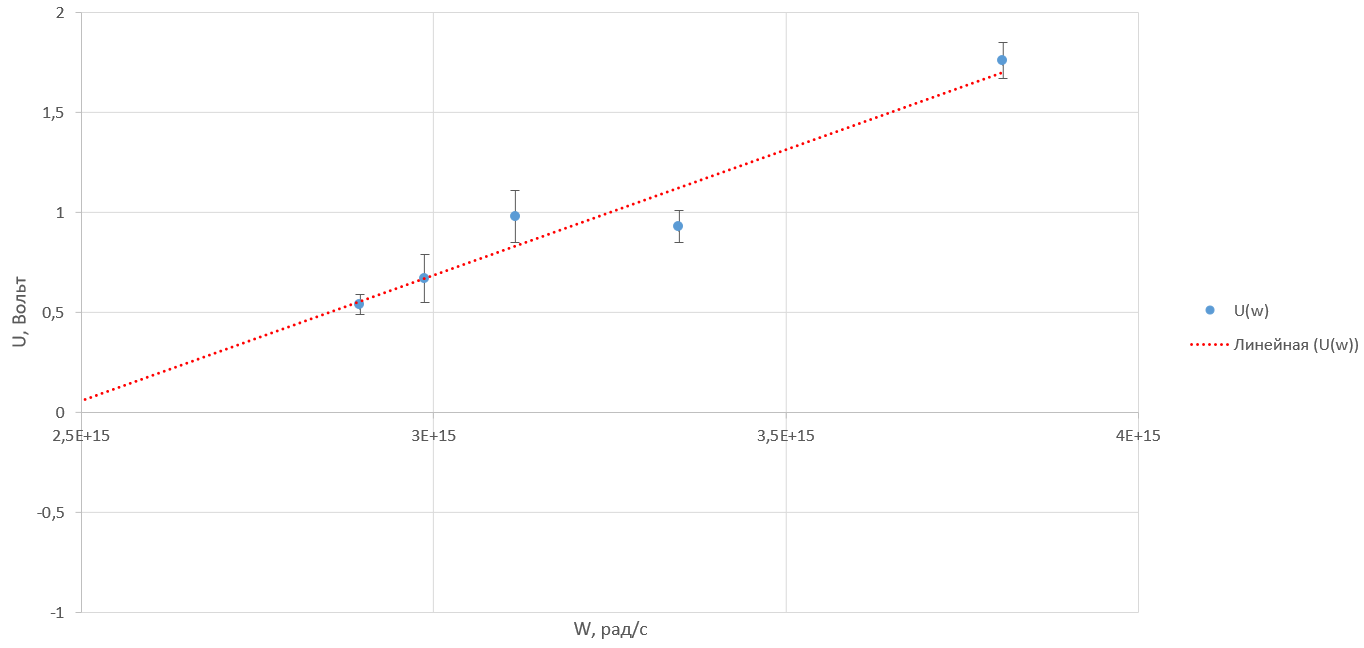
\includegraphics[width=1\textwidth]{2024-09-29_02-12-13.png}
	\label{fig:boiler}
\end{figure}

Уравнение линеаризации:

\begin{equation}
	V_0 = (-1.5 \pm 0.7) + (0.6 \pm 0.2)\cdot 10^{-15} \omega
\end{equation}

Из которого получается постоянная Планка

\begin{equation}
	\hbar = \frac{d V_0}{d \omega} \cdot e \approx (1 \pm 0.3) \cdot 10^{-34} \text{Дж} \cdot \text{c}
\end{equation}

Красная граница спектра и работа выхода:

\begin{equation}
	\omega_k = (2.5 \pm 1.4) \cdot 10^{15} c^{-1}
\end{equation}

\begin{equation}
	W = \hbar \omega_k = 1.6 \pm 0.9 \text{ эВ}
\end{equation}

%\begin{center}
%	\Large $q(T)$
%\end{center}

%\begin{figure}[!h]
%	\centering
%	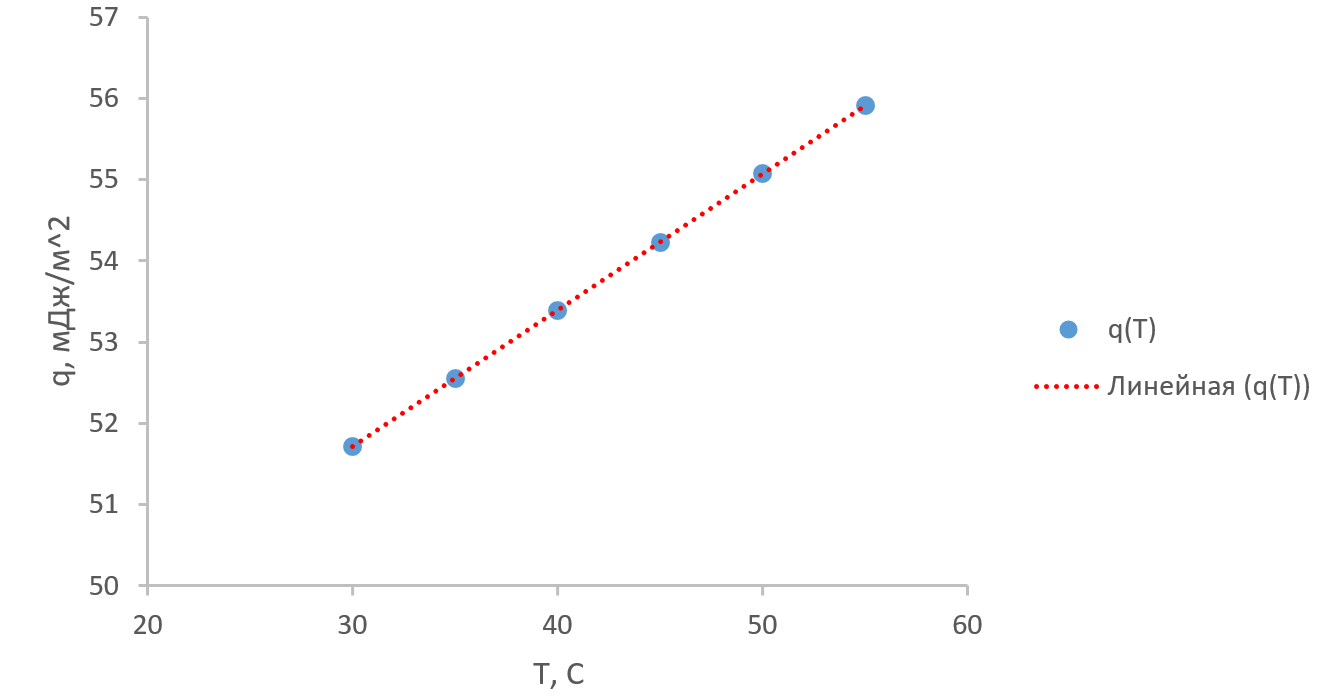
\includegraphics[width=1\textwidth]{2023-02-23_22-23-59.png}
%	\label{fig:boiler}
%\end{figure}

\section{Вывод}

Теория Эйнштейна фотоэффекта подтвердилась, получилось достаточно точно откалибровать прибор, чтобы корректно измерить все теоретические зависимости, которые надлежащим образом были аппроксимированы, что позволило получить точное значение(в рамках погрешности) постоянной Дирака, а также разумное значение работы выхода металла.

\section{Ресурсы}

Расчет по МНК: метод-наименьших-квадратов.рф


\end{problem}
\end{document}